\documentclass[tikz, crop, border = {2pt 2pt 2pt 2pt}]{standalone}

\usetikzlibrary{calc}
\usepackage{concmath-otf}

\begin{document}
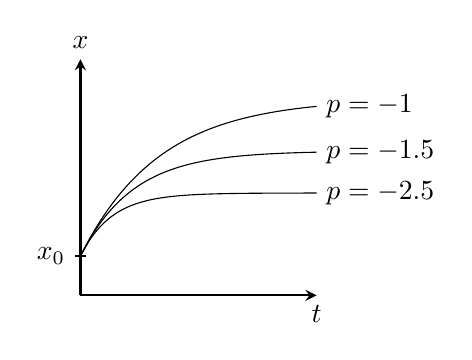
\begin{tikzpicture}
    \draw[-stealth, thick] (0, 0) -- (3, 0) node[below]{$t$};
    \draw[-stealth, thick] (0, 0) -- (0, 3) node[above]{$x$};

    \foreach \x in {-1, -1.5, -2.5} {
        \draw[smooth, variable = \t, domain = 0:3] plot (\t, {0.5 + 2/(\x)*(e^(\x*\t) - 1)}) node[right]{$p = \x$};
    }
    
    \draw (2pt, 0.5) -- ++ (-4pt, 0) node[left]{$x_0$};
\end{tikzpicture}
\end{document}